\documentclass[a4paper]{scrreprt}
 
\usepackage[german]{babel}
\usepackage[utf8]{inputenc}
\usepackage[T1]{fontenc}
\usepackage{ae}
\usepackage[bookmarks,bookmarksnumbered]{hyperref}
 
\begin{document}
 
\title{Pflichtenheft mit LaTeX}
\author{Karl Lorey}
\maketitle
 
% Die abstract-Umgebung kann bei Bedarf aus dem Pflichtenheft entfernt werden
\begin{abstract}
Dies ist ein beispielhaftes Pflichtenheft in \LaTeX. Das Pflichtenheft
beschreibt in konkreter Form, wie der Auftragnehmer die Anforderungen des
Auftraggebers zu lösen gedenkt - das sogenannte wie und womit. Der Auftraggeber
beschreibt vorher im Lastenheft möglichst präzise die Gesamtheit der
Forderungen - was er entwickelt oder produziert haben möchte. Erst wenn der
Auftraggeber das Pflichtenheft akzeptiert, sollte die eigentliche Arbeit beim
Auftragnehmer beginnen.
\vspace{1cm}
 
Quelle: \url{http://de.wikipedia.org/wiki/Pflichtenheft} und Lehrbuch der
Objektmodellierung von Heide Balzert
\vspace{0.5cm}
 
Quellcode: \url{http://www.karllorey.de/informatik-studium/vorlesungen/softwarepraktikum/pflichtenheft-in-latex/}
\end{abstract}
 
% Platzierung des Inhaltsverzeichnisses
\tableofcontents

\chapter{Zielbestimmung}
Dieses Kapitel dient der Bestimmung von Zielen und nicht für deren Verwendung
notwendige Funktionen.
 
\section{Musskriterien}
%blubla Musskriterien: Für das Produkt unabdingbare Leistungen, die in jedem Fall
%erfüllt werden müssen \footnote{gezwungen sein, etwas zu tun (Dies ist eine
%beispielhafte Fußnote).}. Das System ist ohne diese Funktionen für seinen
%gedachten Zweck nicht einsetzbar.

Um dem Ziel, der Erkennung einer handegschriebenen Ziffer, gerecht zu werden, müssen 
folgende Kriterien erfüllt sein:

\begin{itemize}
\item Möglichkeit zur Erfassung einer handgeschriebenen Ziffer in einer Weboberfläche
\item Umwandlung der Eingabeziffer in eine maschinenlesbare Form mithilfe neuronaler Netze
\item Ausgabe der Resultate in einer Weboberfläche
\item Erstellung und Bearbeitung von neuronalen Netzten
\item trainieren der neuronalen Netzten
\item Persistierung von neuronalen Netzen
\end{itemize}
 
\section{Kannkriterien}
%Kannkriterien: Die Erfüllung der Kannkriterien ist erwünscht, jedoch nicht
%unbedingt notwendig. Sie sollten nur angestrebt werden, falls noch ausreichend
%Kapazitäten vorhanden sind.

Sind die Musskriterien erfüllt und noch freie Kapazitäten vorhanden, werden folgende Kriterien bearbeitet:

\begin{itemize}
\item Internationalisierung zur Steigerung der Usability
\item Erschaffung der Möglichkeit verschieden trainierte neuronale Netze auszuwählen
\item Suchfunktion über vorhandene Netze in der Weboberfläche
\end{itemize}

 
\section{Abgrenzungskriterien}
Im späteren Entwicklungszyklus der Anwendung sollen die Funktionalitäten erweitert werden. Denkbar wäre die Möglichkeit
der Eingabe einfacher mathematischer Operationen, welche durch das neuronale Netz erkannt und berechnet werden.

 \chapter{Einsatz}
Der geplante Einsatz des Systems ist die Grundlage für Benutzungsoberfläche und
Qualitätsanforderungen.
 
\section{Anwendungsbereiche}
%Ein Pflichtenheft wird bspw. in einer IT-Abteilung genutzt.

Das System ist über einen, mit dem Internet verbundenen Rechner aufrufbar.
Dadurch kann die Anwendung von allen Personen mit Internetzugang genutzt werden.


 
\section{Zielgruppen}
%Die Zielgruppe besteht also aus Informatikern, die mit der Projektplanung
%beauftragt wurden.

Die größte Zielgruppe ist der Standartnutzer ohne technische Vorkenntnisse, welcher sich für eine Erkennung handschriftlicher Ziffern interessiert.
Da es sich um ein Open-Source Projekt handelt, sollen auch technisch versierte Informatiker angesprochen und zur Teilnahme an der Entwicklung 
der Handschriftserkennung mithilfe neuronaler Netze angeregt werden.

\section{Betriebsbedingungen}
%Betriebsbedingungen: Die Betriebsbedingungen spezifiziert die physikalische
%Umgebung des Systems, die tägliche Betriebszeit, und ob das System ständiger
%Beobachtung durch Bediener ausgesetzt ist, oder ein unbeaufsichtigter Betrieb
%beabsichtigt ist.

Die Grundvorrausetzung zur Inbetriebnahme der Anwendung ist ein Server mit Webanbindung. Auf diesem muss mindestens Java 8 installiert sein.
Zur Persistierung der Daten wird mongoDB der Version 3.2.10 verwendet. Der Betrieb der Datenbank muss dauerhaft gewährleistet und die Daten
jederzeit vom Server abrufbar sein. Es wird ein unbeaufsichtiger Betrieb beabsichtigt. 

 
\chapter{Umgebung}
 
\section{Software}
%Software: Gibt an, welche Software zum Betrieb vorhanden sein muss. Eine
%Aufteilung für Server und Client ist ggf. sinnvoll. Weiterhin sind unbedingt die
%kleinsten benötigten Versionsnummern anzugeben.
\subsection {Für Endanwender}

\begin{itemize}
\item aktueller Internet Browser
\end{itemize}

\subsection	{Für Entwickler}

\begin{itemize}
\item Java 8
\item Apache Maven 3.3.9
\item Spring Framework 1.4.1
\item Vaadin 7.7.3
\item FasterXML 0.6.2
\item Lombok 1.16.10
\item TestNG 6.9.13.6
\item Mockito 2.0.2 beta
\item dozer 5.5.1
\item Apache Commons-io 2.5
\end{itemize}
 
\section{Hardware}

\begin{itemize}
\item Application-Server mit Internetanbindung
\end{itemize} 

\section{Orgware}
%Orgware: Angabe der organisatorische Rahmenbedingungen, die vor Projektstart
%erfüllt sein müssen.
\begin{itemize}
\item Web-Repository GitHub zur Versionsverwaltung
\item gitter.im zur internen Kommunikation 
\end{itemize}

\section{Funktionalität}

\subsection{Programmfunktionalitäten}
\subsubsection{Funktionsübersicht}

\textbf{/F101/} Es gibt einen Zeichenbereich, in den freihändisch (z.B. mittels Maus) eine Ziffer geschrieben werden kann.\\[-0.2cm]

\textbf{/F102/} Ein neuronales Netz berechnet aus dem gezeichneten Bild der Ziffer die Ziffer in maschinenlesbarer Form und gibt das Ergebnis auf der Seite aus. \\[-0.2cm]

\textbf{/F103/} Die Berechnung wird wahlweise synchron durchgeführt oder manuell angestoßen.\\[-0.2cm]

\textbf{/F104/} Auf der Anwendungsseite für den Endanwender sollen bei Bedarf Informationen über das verwendete neuronale Netz eingeblendet werden.\\[-0.2cm]

\textbf{/F105/} Es ist möglich, aus einer Liste eines von mehreren möglichen neuronalen Netzen auszuwählen bzw. nach einem bestimmten Netz zu suchen. \\[-0.2cm]

\textbf{/F106/} Auf der Anwendungsseite werden Statusinformationen (z.B. zum Stand der Berechnung) ausgegeben. \\[-0.2cm]

\textbf{/F201/} Jedes neuronale Netz kann mit dem Gradienten-Abstieg-Algorithmus trainiert werden. Dabei sind die Trainingsparameter \emph{Lernrate}, \emph{Stapelgröße}, \emph{Anzahl der Trainingsbilder} und \emph{Zyklenanzahl} frei wählbar. Als Trainingsbasis ist die MNIST-Datenbank\footnote{Die MNIST-Database ist eine Sammlung von 60000 Trainingsbildern handgeschriebener Ziffern und zusätzlichen 10000 Testbildern, siehe auch \url{http://yann.lecun.com/exdb/mnist/}. \label{footnote_mnist}} zu verwenden.

\textbf{/F202/} Das Training kann manuell gestartet und gestoppt werden.\\[-0.2cm]

\textbf{/F203/} Der Nutzer soll über eine Ausgabe-Konsole über den Trainingsstand und die Genauigkeit des neuronalen Netzes informiert werden -- als Testbasis ist die MNIST-Testdatenbank zu verwenden.

\textbf{/F204/} Ein trainiertes neuronales Netz kann bei Bedarf gespeichert oder verworfen werden. Wird das trainierte Netz, z.B. durch die Auswahl eines anderen neuronalen Netzes, verworfen, ist dies auf der Konsole auszugeben. \\[-0.2cm]

\textbf{/F301/} Die Metadaten (Name, Beschreibung) eines neuronalen Netzes sollen konfigurierbar sein.\\[-0.2cm]

\textbf{/F302/} Die Topologie des Netzes sowie die Eigenschaften von Knoten und Knotenverbindungen sollen über eine JSON-Struktur bearbeitbar sein.\footnote{Es wird keine Validierung des eingegebenen JSON-Strings vorgenommen. Im Rahmen des Projektes wird davon Ausgegangen, dass der Administrator weiß, welche Netztopologien zulässig sind -- z.B. eine Eingabeschicht mit $28 \times 28$ Eingabeknoten und eine Ausgabeschicht mit 10 Ausgabeknoten.}\\[-0.2cm]

\textbf{/F303/} Die in /F301/ und /F302/ am neuronalen Netz vorgenommenen Änderungen sollen gespeichert werden können.\\[-0.2cm]

\textbf{/F304/} Es ist möglich ein neues neuronales Netz anzulegen.

\newpage
\subsubsection{Arbeitsflüsse}

\textbf{Aktivitätsdiagramm aus Administrationssicht.} Der Administrationsbereich der Anwendung setzt sich aus zwei Unterseiten zusammen, nämlich einer Seite für die Konfiguration der Trainingsparameter (vgl. Abb. \ref{ui-train}) sowie für die Bearbeitung der neuronalen Netze (vgl. Abb. \ref{ui-crud}). Der Arbeitsfluss zwischen beiden Seiten ist im folgenden Aktivitätsdiagramm dargestellt.

\begin{figure}[H]
\begin{center}
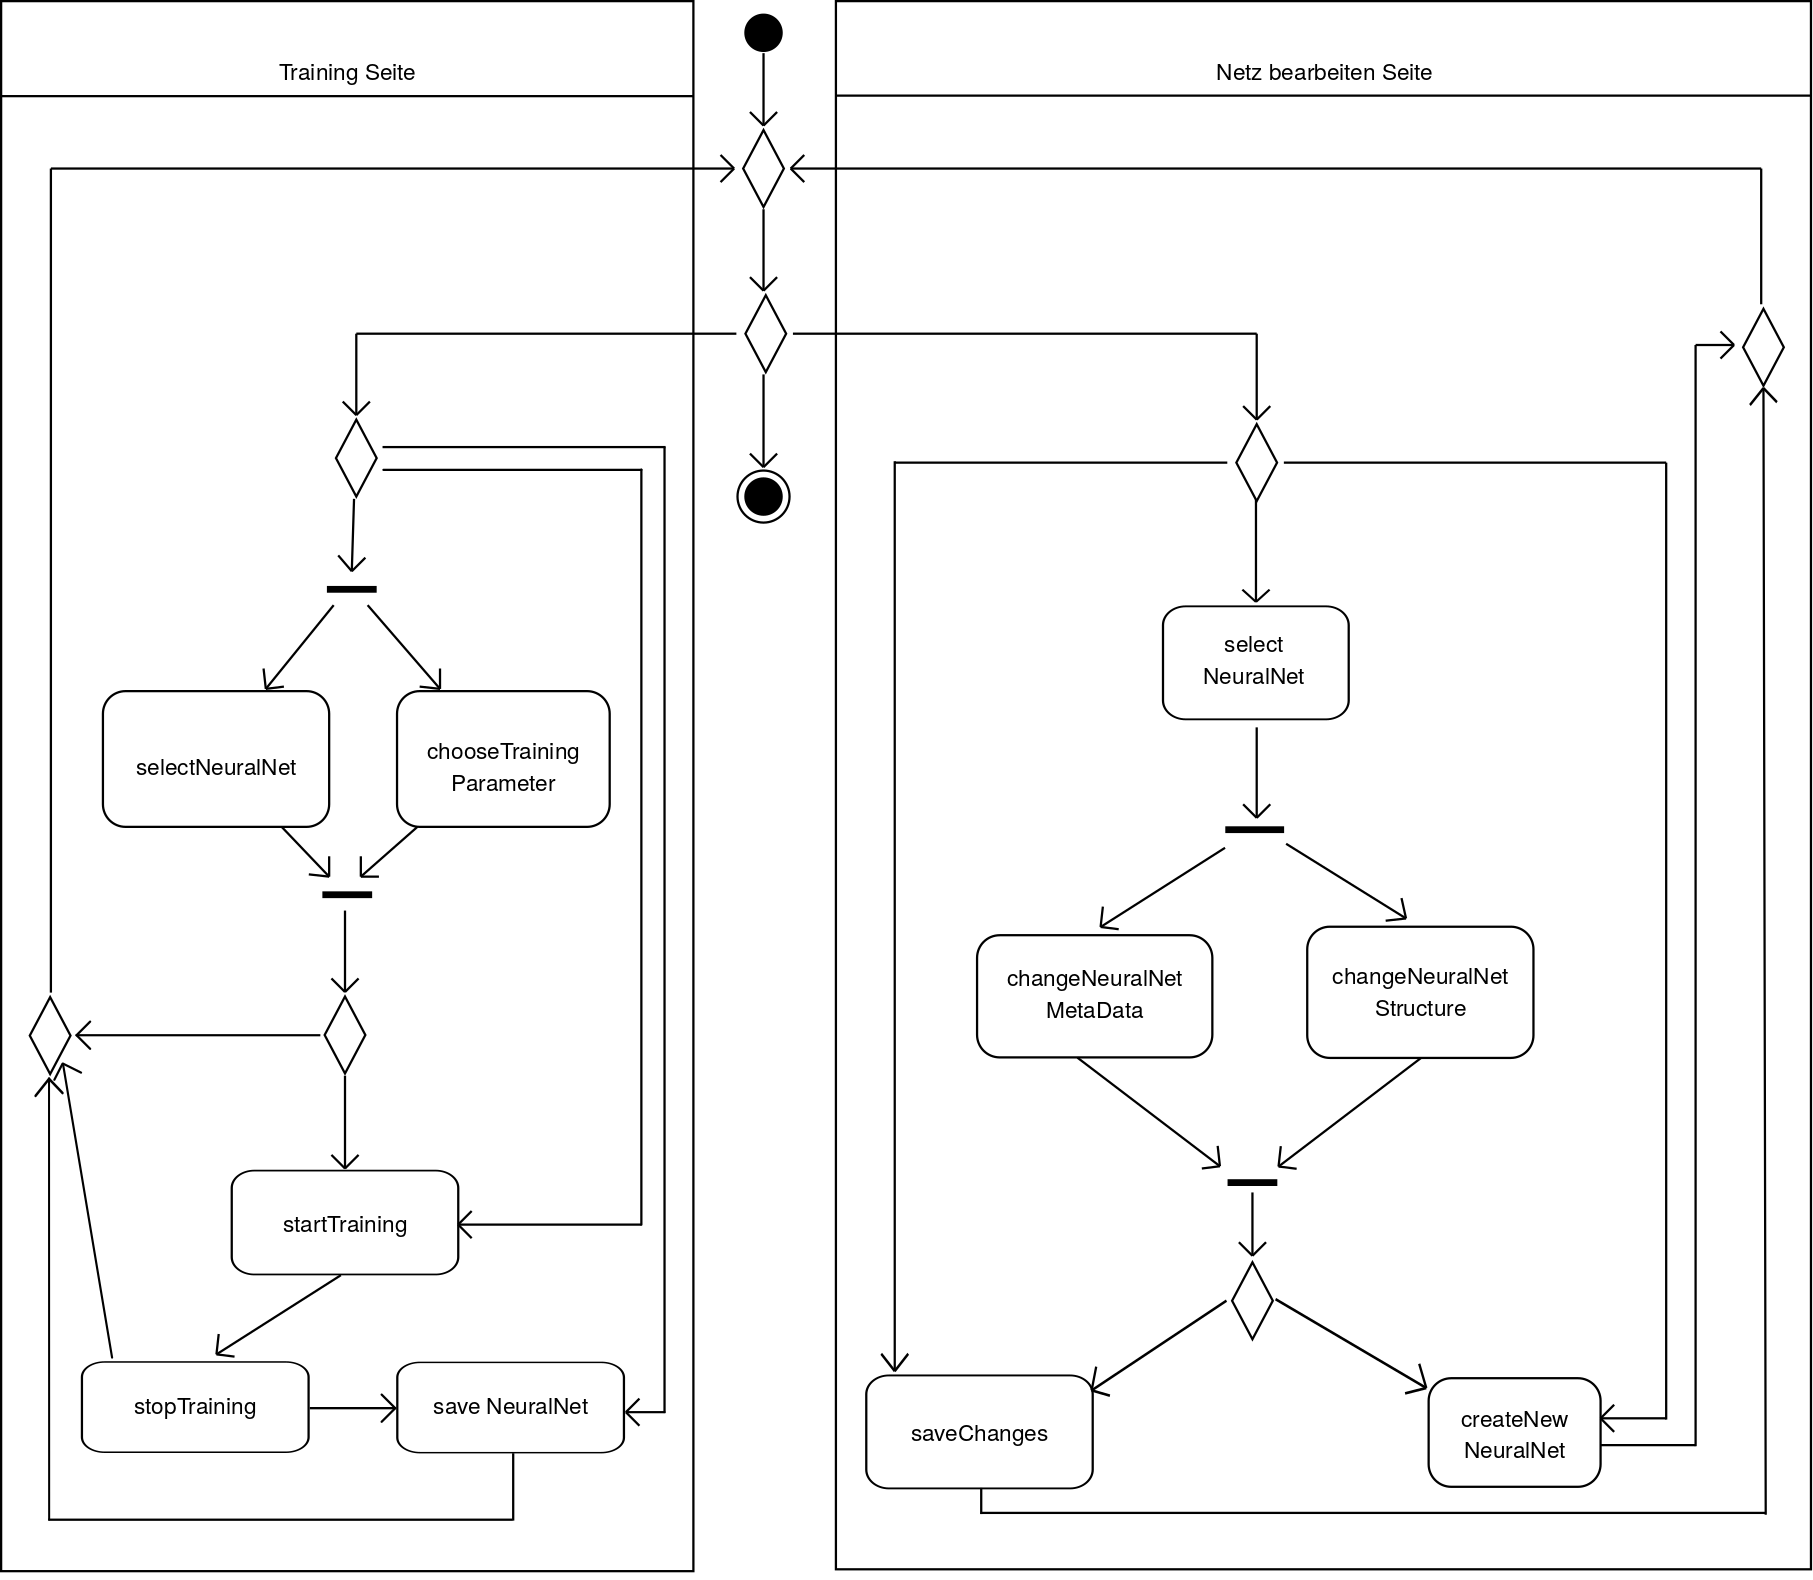
\includegraphics[width=\textwidth]{Abbildungen/UML/jan/trainingConfigAD.png}
\caption{Aktivitätsdiagramm für die Verwendung des Programmes im Administrationsbereich.}
\label{fig_trainingConfigAD}
\end{center}
\end{figure}

\textbf{Aktivitätsdiagramm aus Anwendersicht.} Die folgende Abbildung beschreibt den grundlegenden Arbeitsfluss vom Starten der Anwendung, bis hin zur Ausgabe des Resultates.
\begin{figure}[H]
\begin{center}
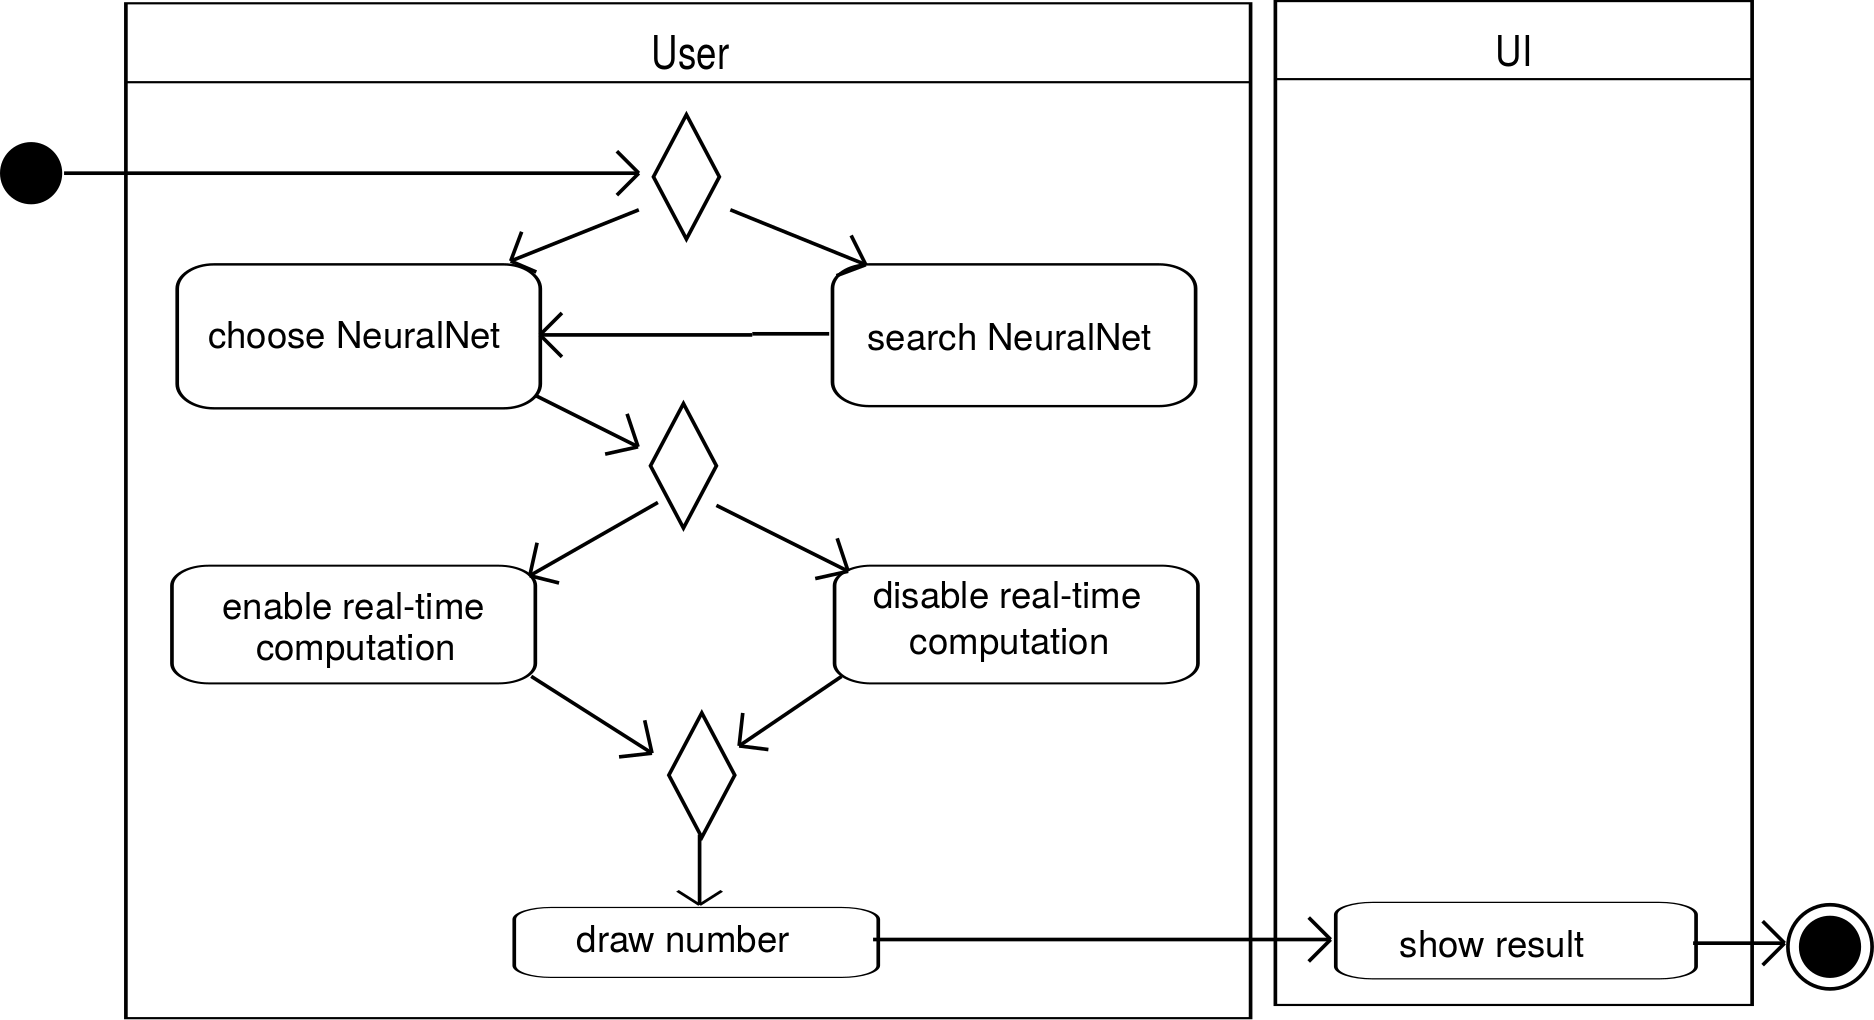
\includegraphics[width=\textwidth]{Abbildungen/UML/uml_ronny/AD_UI.png}
\caption{Aktivitätsdiagramm für die Verwendung des Programmes aus Anwendersicht.}
\label{fig_AD_UI}
\end{center}
\end{figure}


\subsection{Globale Programmarchitektur}

Zur Entkopplung einzelner Module und leichteren Wartbarkeit verwendet die Anwendung, wie in Abb. \ref{Drei-Schichten-Architektur} zu sehen, eine Drei-Schichten Architektur bestehend aus Nutzeroberfläche, Business-Schicht und Daten-Schicht.
\begin{figure}[H]
\begin{center}
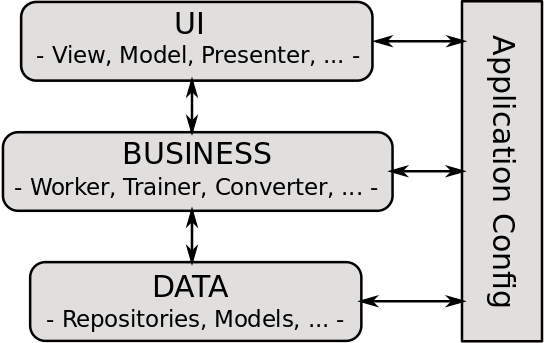
\includegraphics[width=10cm]{Abbildungen/UML/jan/SchichtenModel.png}
\caption{Drei-Schichten-Architektur} 
\label{Drei-Schichten-Architektur}
\end{center}
\end{figure}

Die Nutzeroberfläche dient der Nutzerinteraktion und der Darstellung der eingegebenen sowie verarbeiteten Daten. Sie implementiert dabei das Model-View-Presenter Muster. Für dieses Oberflächenarchitekturmusters sind in Abb. \ref{mvp} die Abhängigkeiten der einzelnen Komponenten untereinander zu sehen.

\textbf{View.} Der View ist nur der Presenter bekannt. Die Funktionalität wird über Schnittstellen festgelegt. Vorteile sind Austausch- und Testbarkeit. Interagiert der Nutzer mit der Oberfläche werden Nachrichten an den Presenter versendet.

\textbf{Presenter.} Der Presenter ist das Bindeglied zwischen Ansicht und Model. Es empfängt Nachrichten der View und verarbeitet diese. Eine erfolgte Aktion könnte zum Beispiel das Laden eines Datensatzes sein. Über das Model werden die Daten bezogen und die View anschließend zur Anzeige deren veranlasst. Der Presenter kennt nur die Schnittstelle zur View, sodass für sein Funktionieren die konkrete Realisierung einer View irrelevant ist.

\textbf{Model.} Das Model ist in unserem Anwendungsfall die Zugriffsschicht auf Geschäftslogik und Daten. Es wird abgebildet über die Businessschicht und deren Workerklassen. Es kennt weder den Presenter noch die View.

\begin{figure}[H]
	\begin{center}
		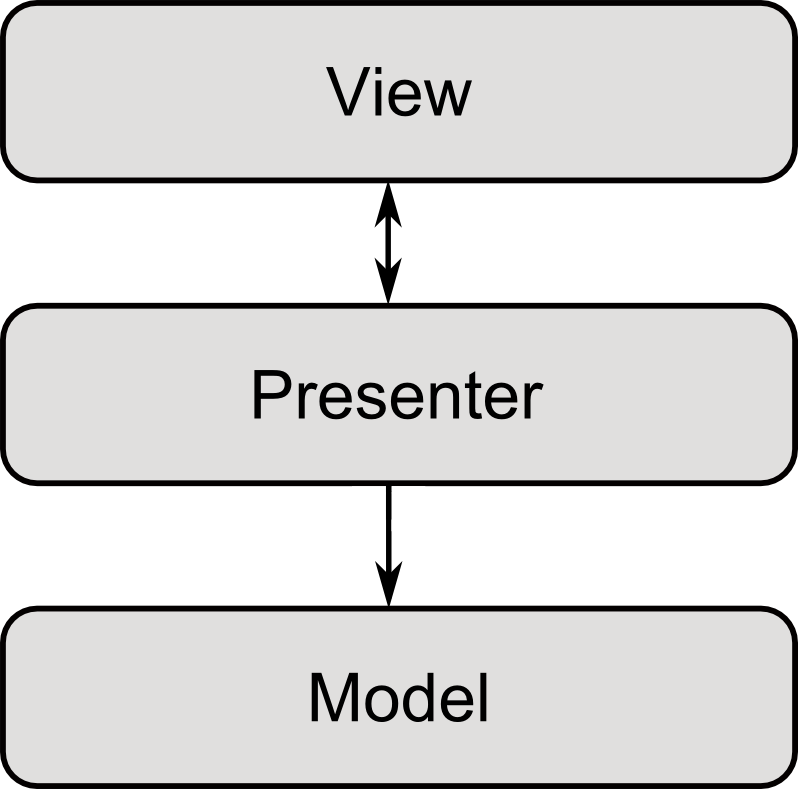
\includegraphics[width=7cm]{Abbildungen/UML/daniel/MVP.png}
		\caption{Model-View-Presenter} 
		\label{mvp}
	\end{center}
\end{figure}

In Abb. \ref{mvp-exemplarisch} ist der vereinfachte exemplarische Aufbau des MVP-Musters zu sehen. Zu beachten ist, dass Interfaces in diesem Diagramm nicht dargestellt sind. Über die abstrakten Klassen BaseView und BasePresenter werden Funktionalitäten bereitgestellt, die in mehreren Ansichten gebraucht werden. Als Beispiel dient die Ziffernerkennungs-Oberfläche. Sie stellt verschiedene Zugriffsmöglichkeiten, wie das Setzen eines Netz-Datensatzes oder des Ergebnisses einer Erkennung, bereit. Die Methoden \textit{setSearchResult} der View und \textit{searchNN} stellen beispielsweise die Möglichkeit zur Suche nach Netzen und deren Anzeige zur Verfügung. Der Presenter hat über die Service-Klasse Zugriff auf die verschiedenen Elemente der Businessschicht. 

\begin{figure}[H]
	\centering
	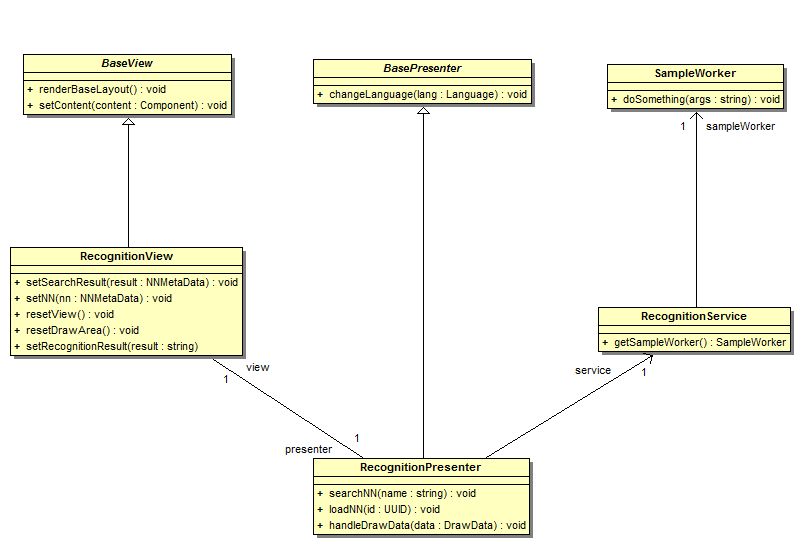
\includegraphics[width=1\textwidth]{Abbildungen/UML/daniel/Klassendiagramm-MVP.png}
	\caption{Exemplarisches Klassendiagramm MVP-Muster}
	\label{mvp-exemplarisch}
\end{figure}


In der Business-Schicht werden alle anschließend fachspezifischen Verarbeitungen vorgenommen. Hierunter fallen beispielsweise die Vorwärtsberechnung sowie das Training eines künstlichen neuronalen Netzes oder die Konvertierung von Daten. Dazu werden für jede Entität spezifische Worker-Klassen bereitgestellt, die diese Aufgaben durchführen können. Abb. \ref{CrudMin} visualisiert diesen Zusammenhang. Der generische Crudworker stellt die allgemeine Funktionalität zur Verfügung. Darüber hinausgehende Anforderungen an den Worker müssen in abgeleiteten Kindklassen implementiert werden.

\begin{figure}[H]
\begin{center}
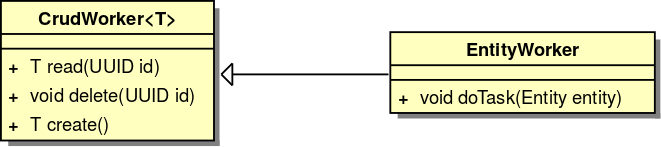
\includegraphics[width=10cm]{Abbildungen/UML/jan/workerClassDiagramm.png}
\caption{Klassendiagramm generischer CrudWorker und beispielhaft ableitender Worker}
\label{CrudMin}
\end{center}
\end{figure}

Als unterste Schicht der Anwendung dient die Daten-Schicht der Persistierung von Daten. Hierfür stehen ihr diverse, von CRUD-Workern angesprochene Repositories zur Verfügung, die je nach Bedarf Daten (hier im Wesentlichen das neuronale Netz) in eine Datenbank oder externe Dateien schreiben können.

In den nächsten Unterabschnitten folgt die ausführliche Beschreibung und geplante Umsetzung der von der Anwendung zu erbringenden Funktionalitäten.  

\subsection{Sequenz- und Klassendiagramme}
\subsubsection{Anwendersicht}

\textbf{/F102/}
\vspace{-0.4cm}
\begin{figure}[H]
\begin{center}
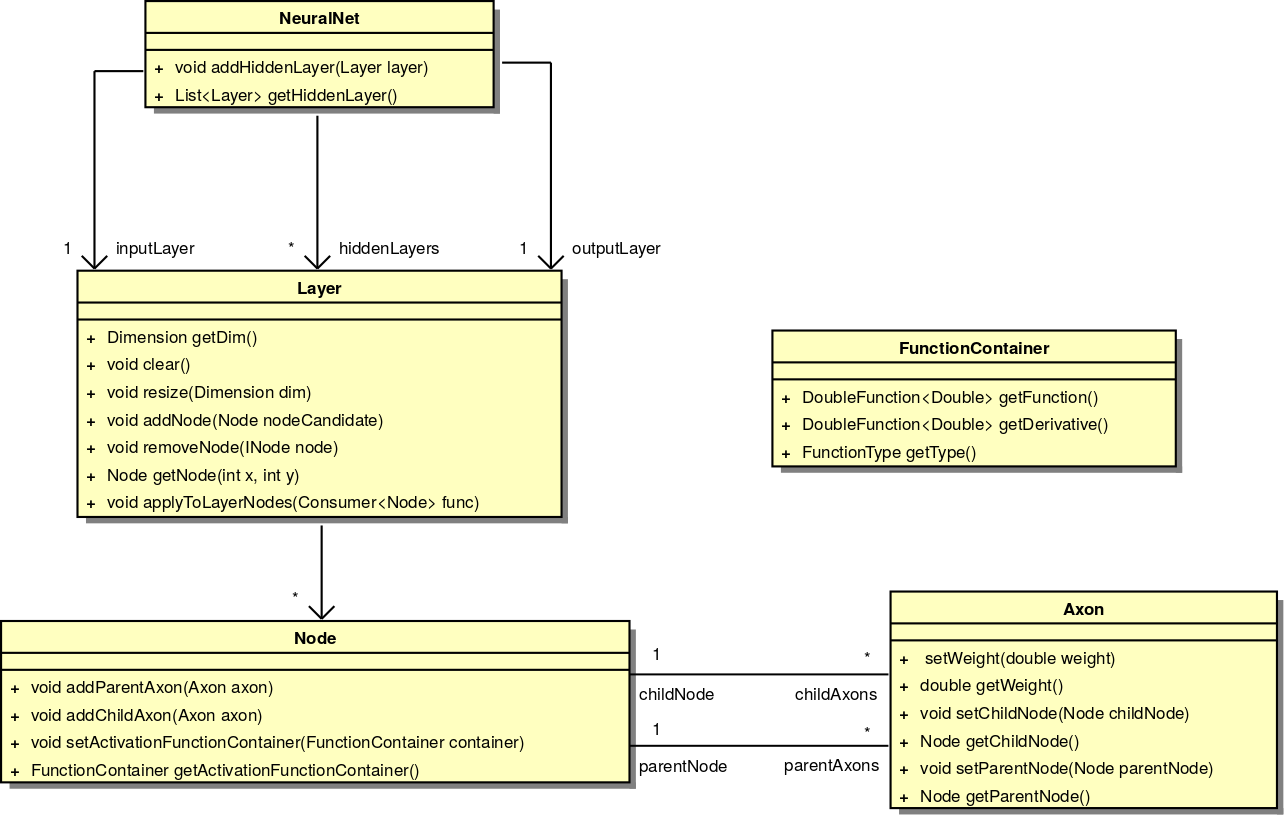
\includegraphics[width=\textwidth]{Abbildungen/UML/uml_ronny/neuralNetKlassenDiagramm.png}
\caption{Klassendiagramm Aufbau und Struktur eines neuralen Netzes}
\label{fig_cdNet}
\end{center}
\end{figure}
\vspace{-0.5cm}
\begin{figure}[H]
\begin{center}
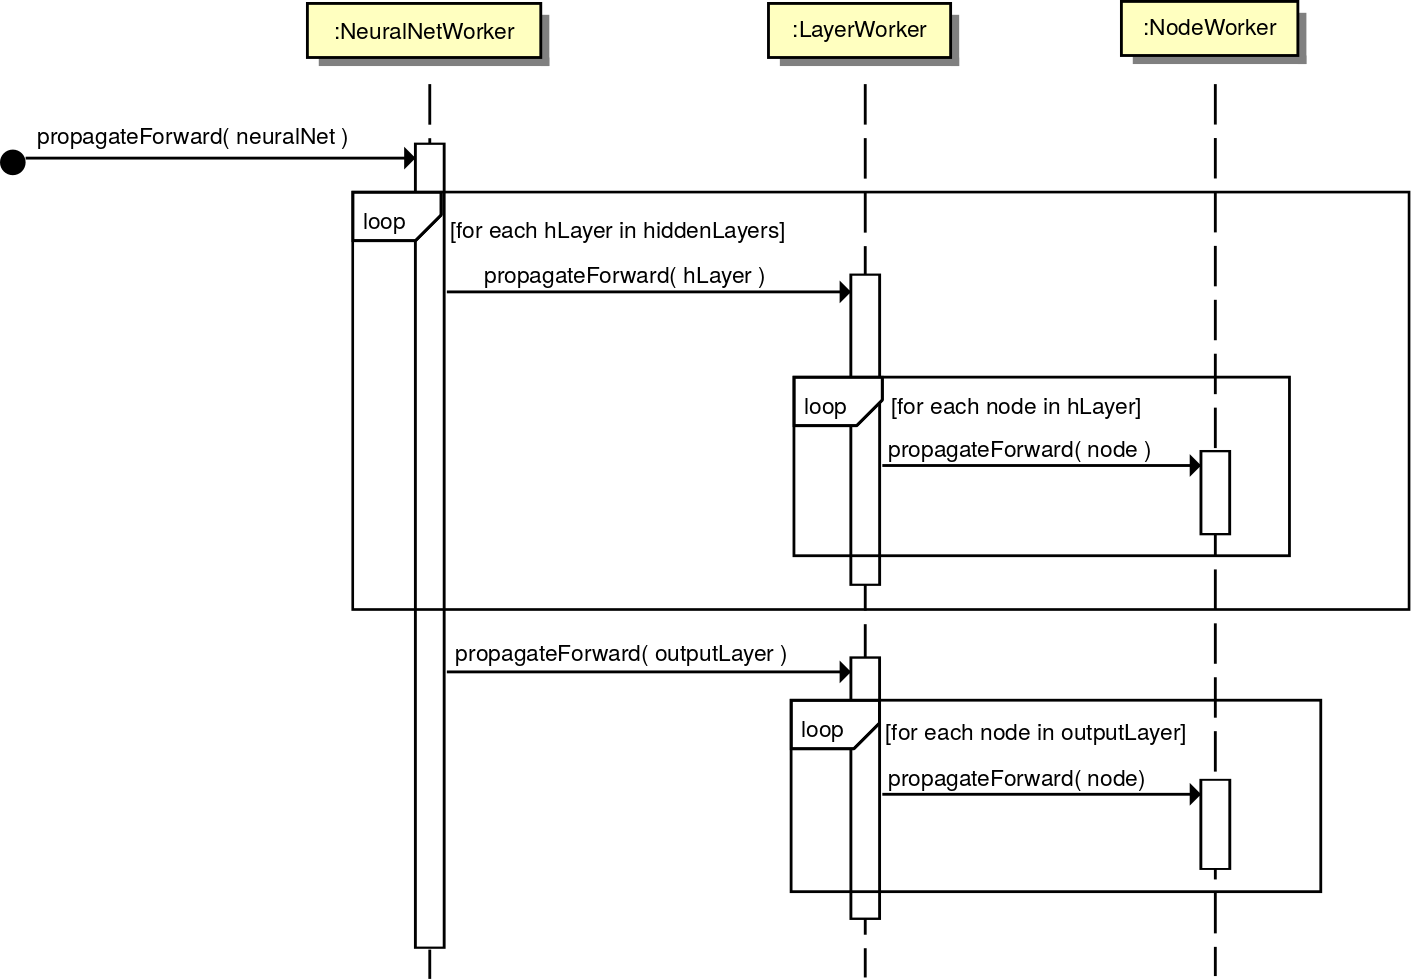
\includegraphics[width=13.5cm]{Abbildungen/UML/uml_ronny/forwardWorkerSequenzDiagramm.png}
\caption{Sequenzdiagramm Vorwärtsberechnung im neuralen Netz}
\label{fig_sdPropForw}
\end{center}
\end{figure}

\begin{figure}[H]
\begin{center}
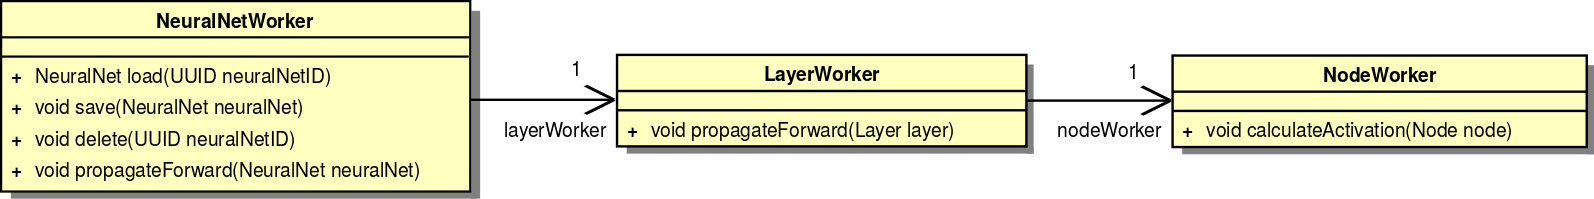
\includegraphics[width=\textwidth]{Abbildungen/UML/uml_ronny/workerKlassenDiagramm.png}
\caption{Klassendiagramm Delegation von speziellen Berechnungen an zusätzliche Worker}
\label{fig_cdWorkerAndSubWorker}
\end{center}
\end{figure}

\subsubsection{Administrationssicht}

\textbf{/F201/} Das Training eines neuronalen Netzes erfolgt mit Hilfe des Gradienten-Abstieg-Algorithmus. Durch den Vergleich von tatsächlicher Netzwerkausgabe zur erwarteten Ausgabe werden dabei beginnend beim Ausgabelayer sukzessive Anpassungen an den Netzwerkknoten und Netzwerkaxon vorgenommen. Für jede Abstraktionstufe des neuronalen Netzes wird dabei ein eigener Trainer angelegt, der für die Rückwärtspropagierung des Ausgabefehlers zuständig ist.\\[-0.5cm]
\begin{figure}[H]
\begin{center}
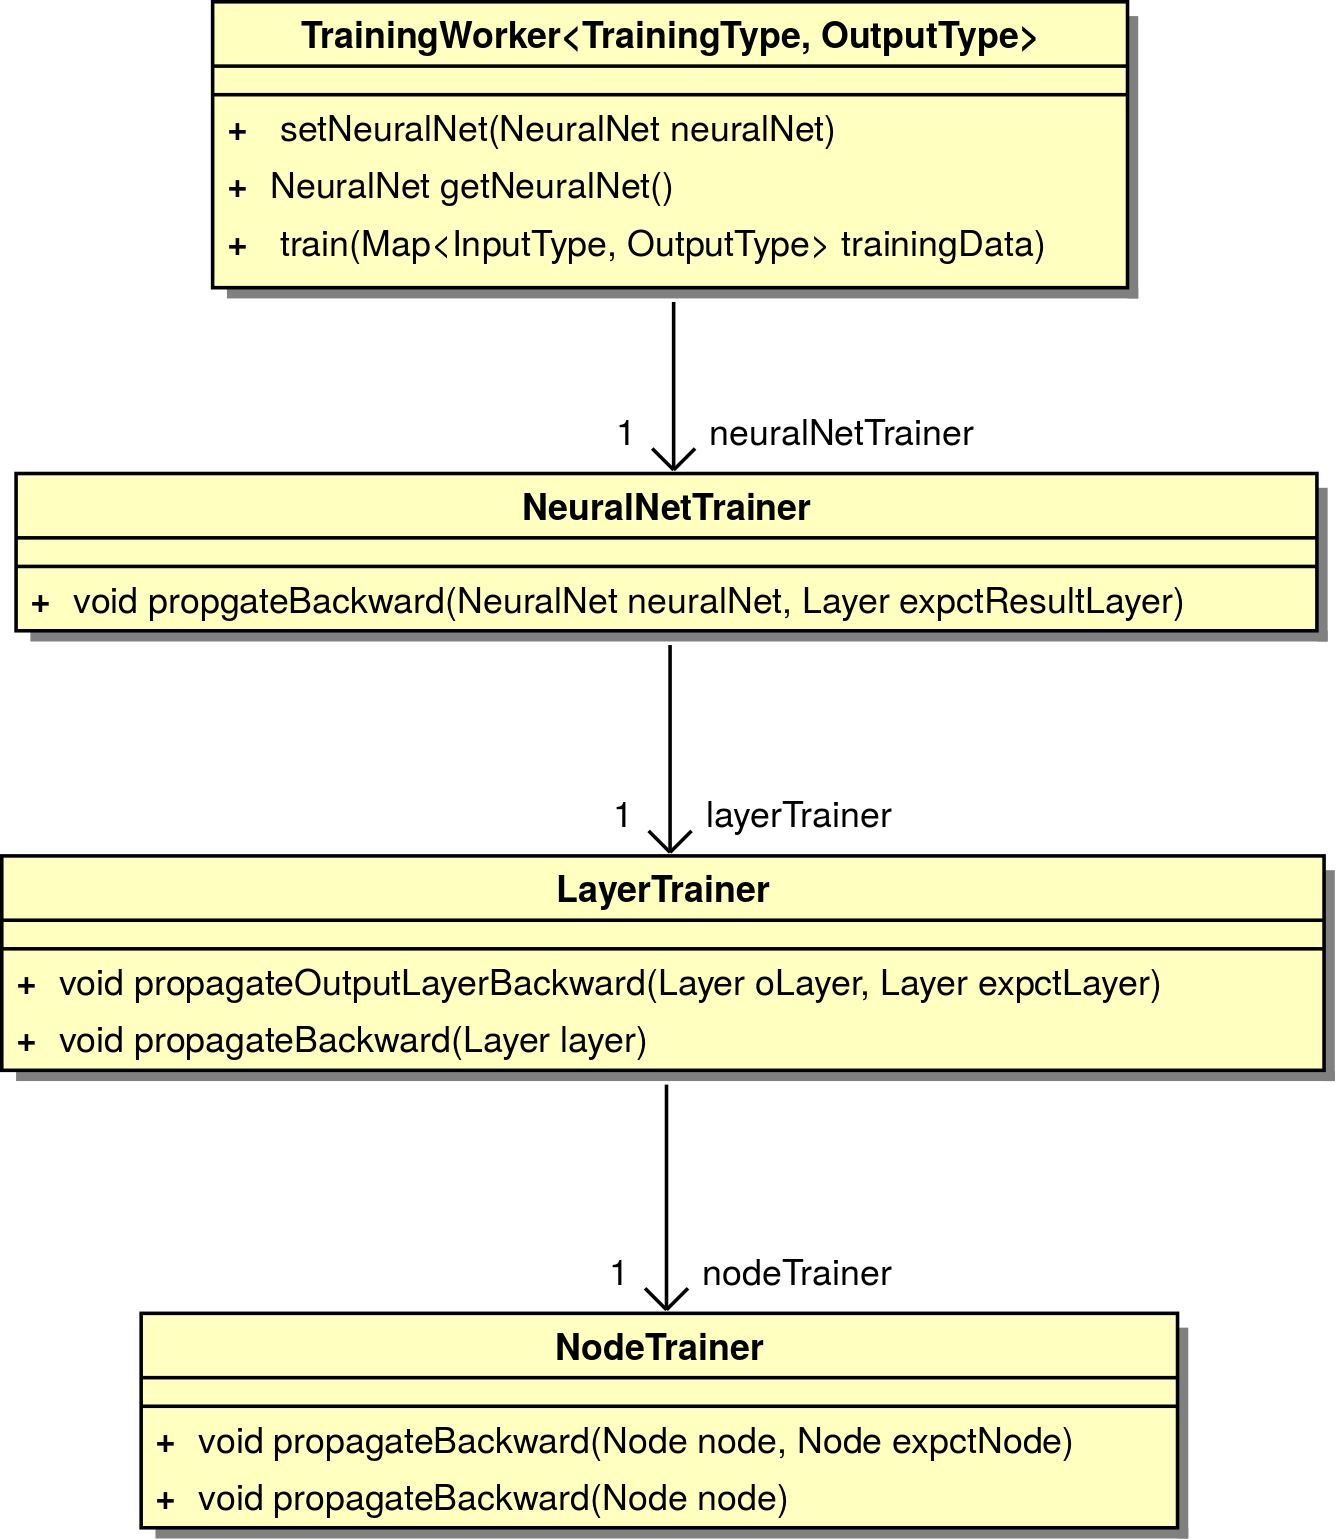
\includegraphics[width=10cm]{Abbildungen/UML/jan/trainerCD.png}
\caption{Klassendiagramm der Trainingsworker für das neuronale Netz, Layer und Nodes.}
\label{fig_cdTraining}
\end{center}
\end{figure}
\newpage
Der Ablauf eines Trainingdurchlaufs stellt sich als Sequenzdiagramm wie folgt dar:
\begin{figure}[H]
\begin{center}
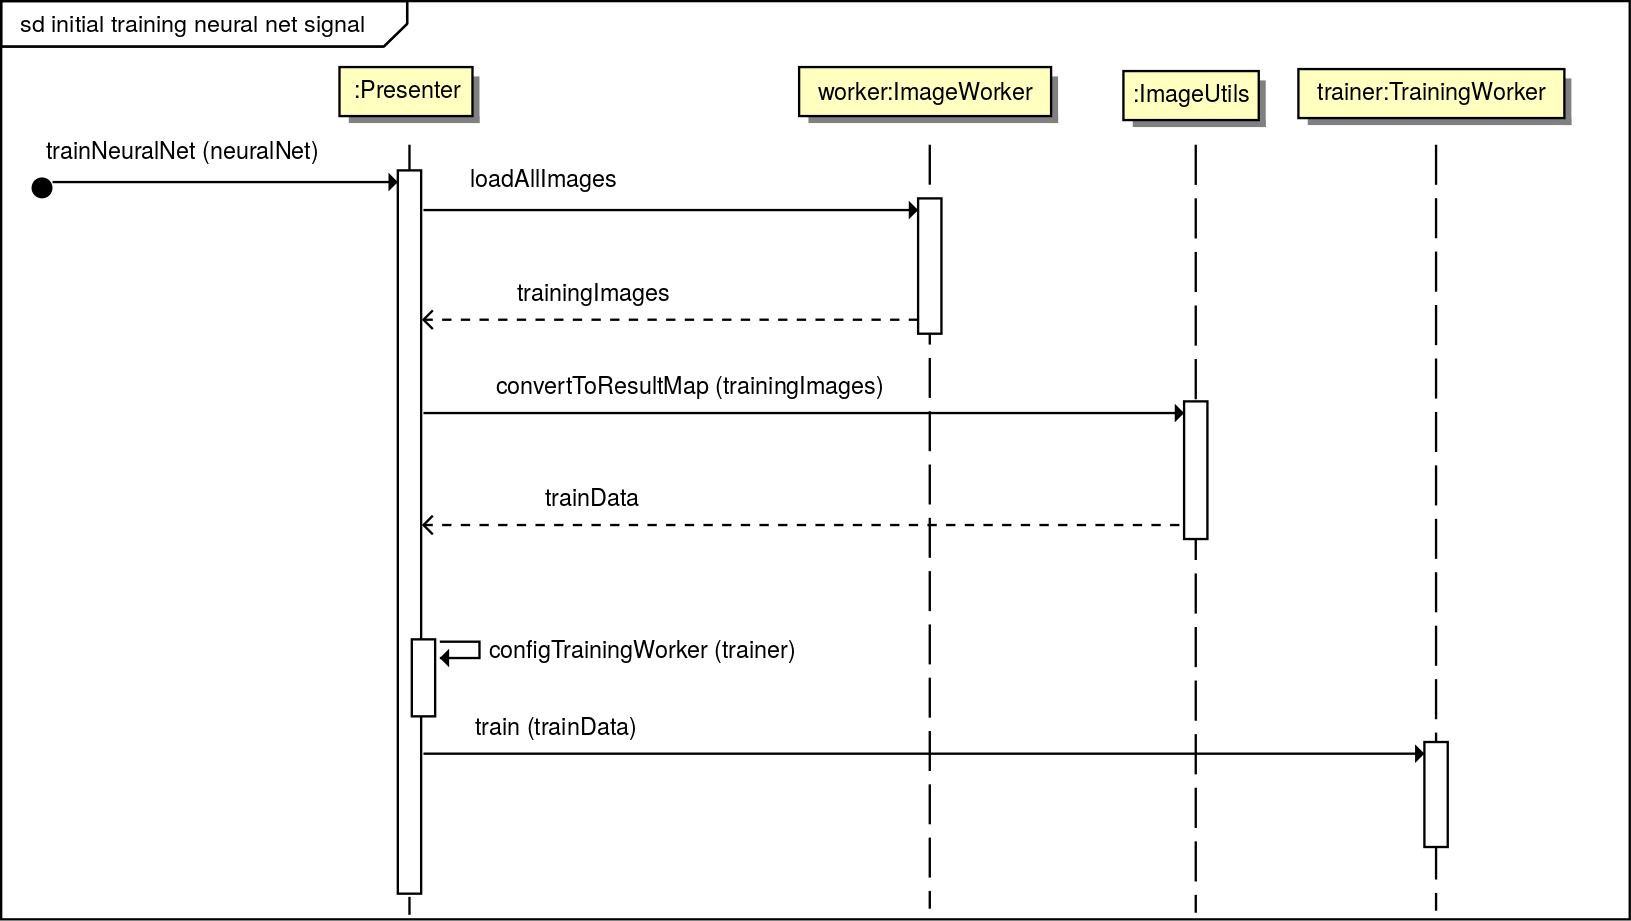
\includegraphics[width=14.2cm]{Abbildungen/UML/jan/trainNeuralNet.png}
\caption{Sequenzdiagramm zum Trainingsprozess beginnend am Presenter.}
\label{fig_sdTraining}
\end{center}
\end{figure}
\begin{figure}[H]
\begin{center}
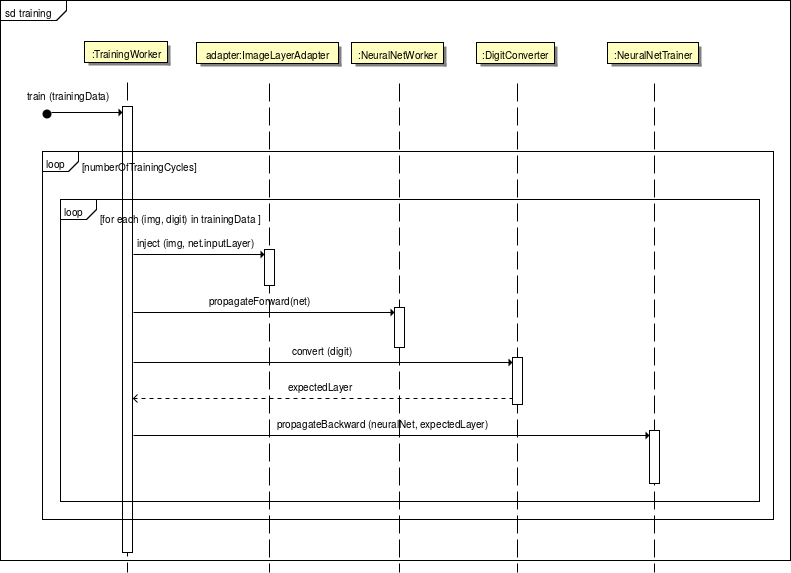
\includegraphics[width=14.2cm]{Abbildungen/UML/jan/trainDetailed1.png}
\caption{Sequenzdiagramm für Trainingsprozess im Trainingsworker.}
\label{fig_sdTraining}
\end{center}
\end{figure}
\vspace{-0.5cm}
\begin{figure}[H]
\begin{center}
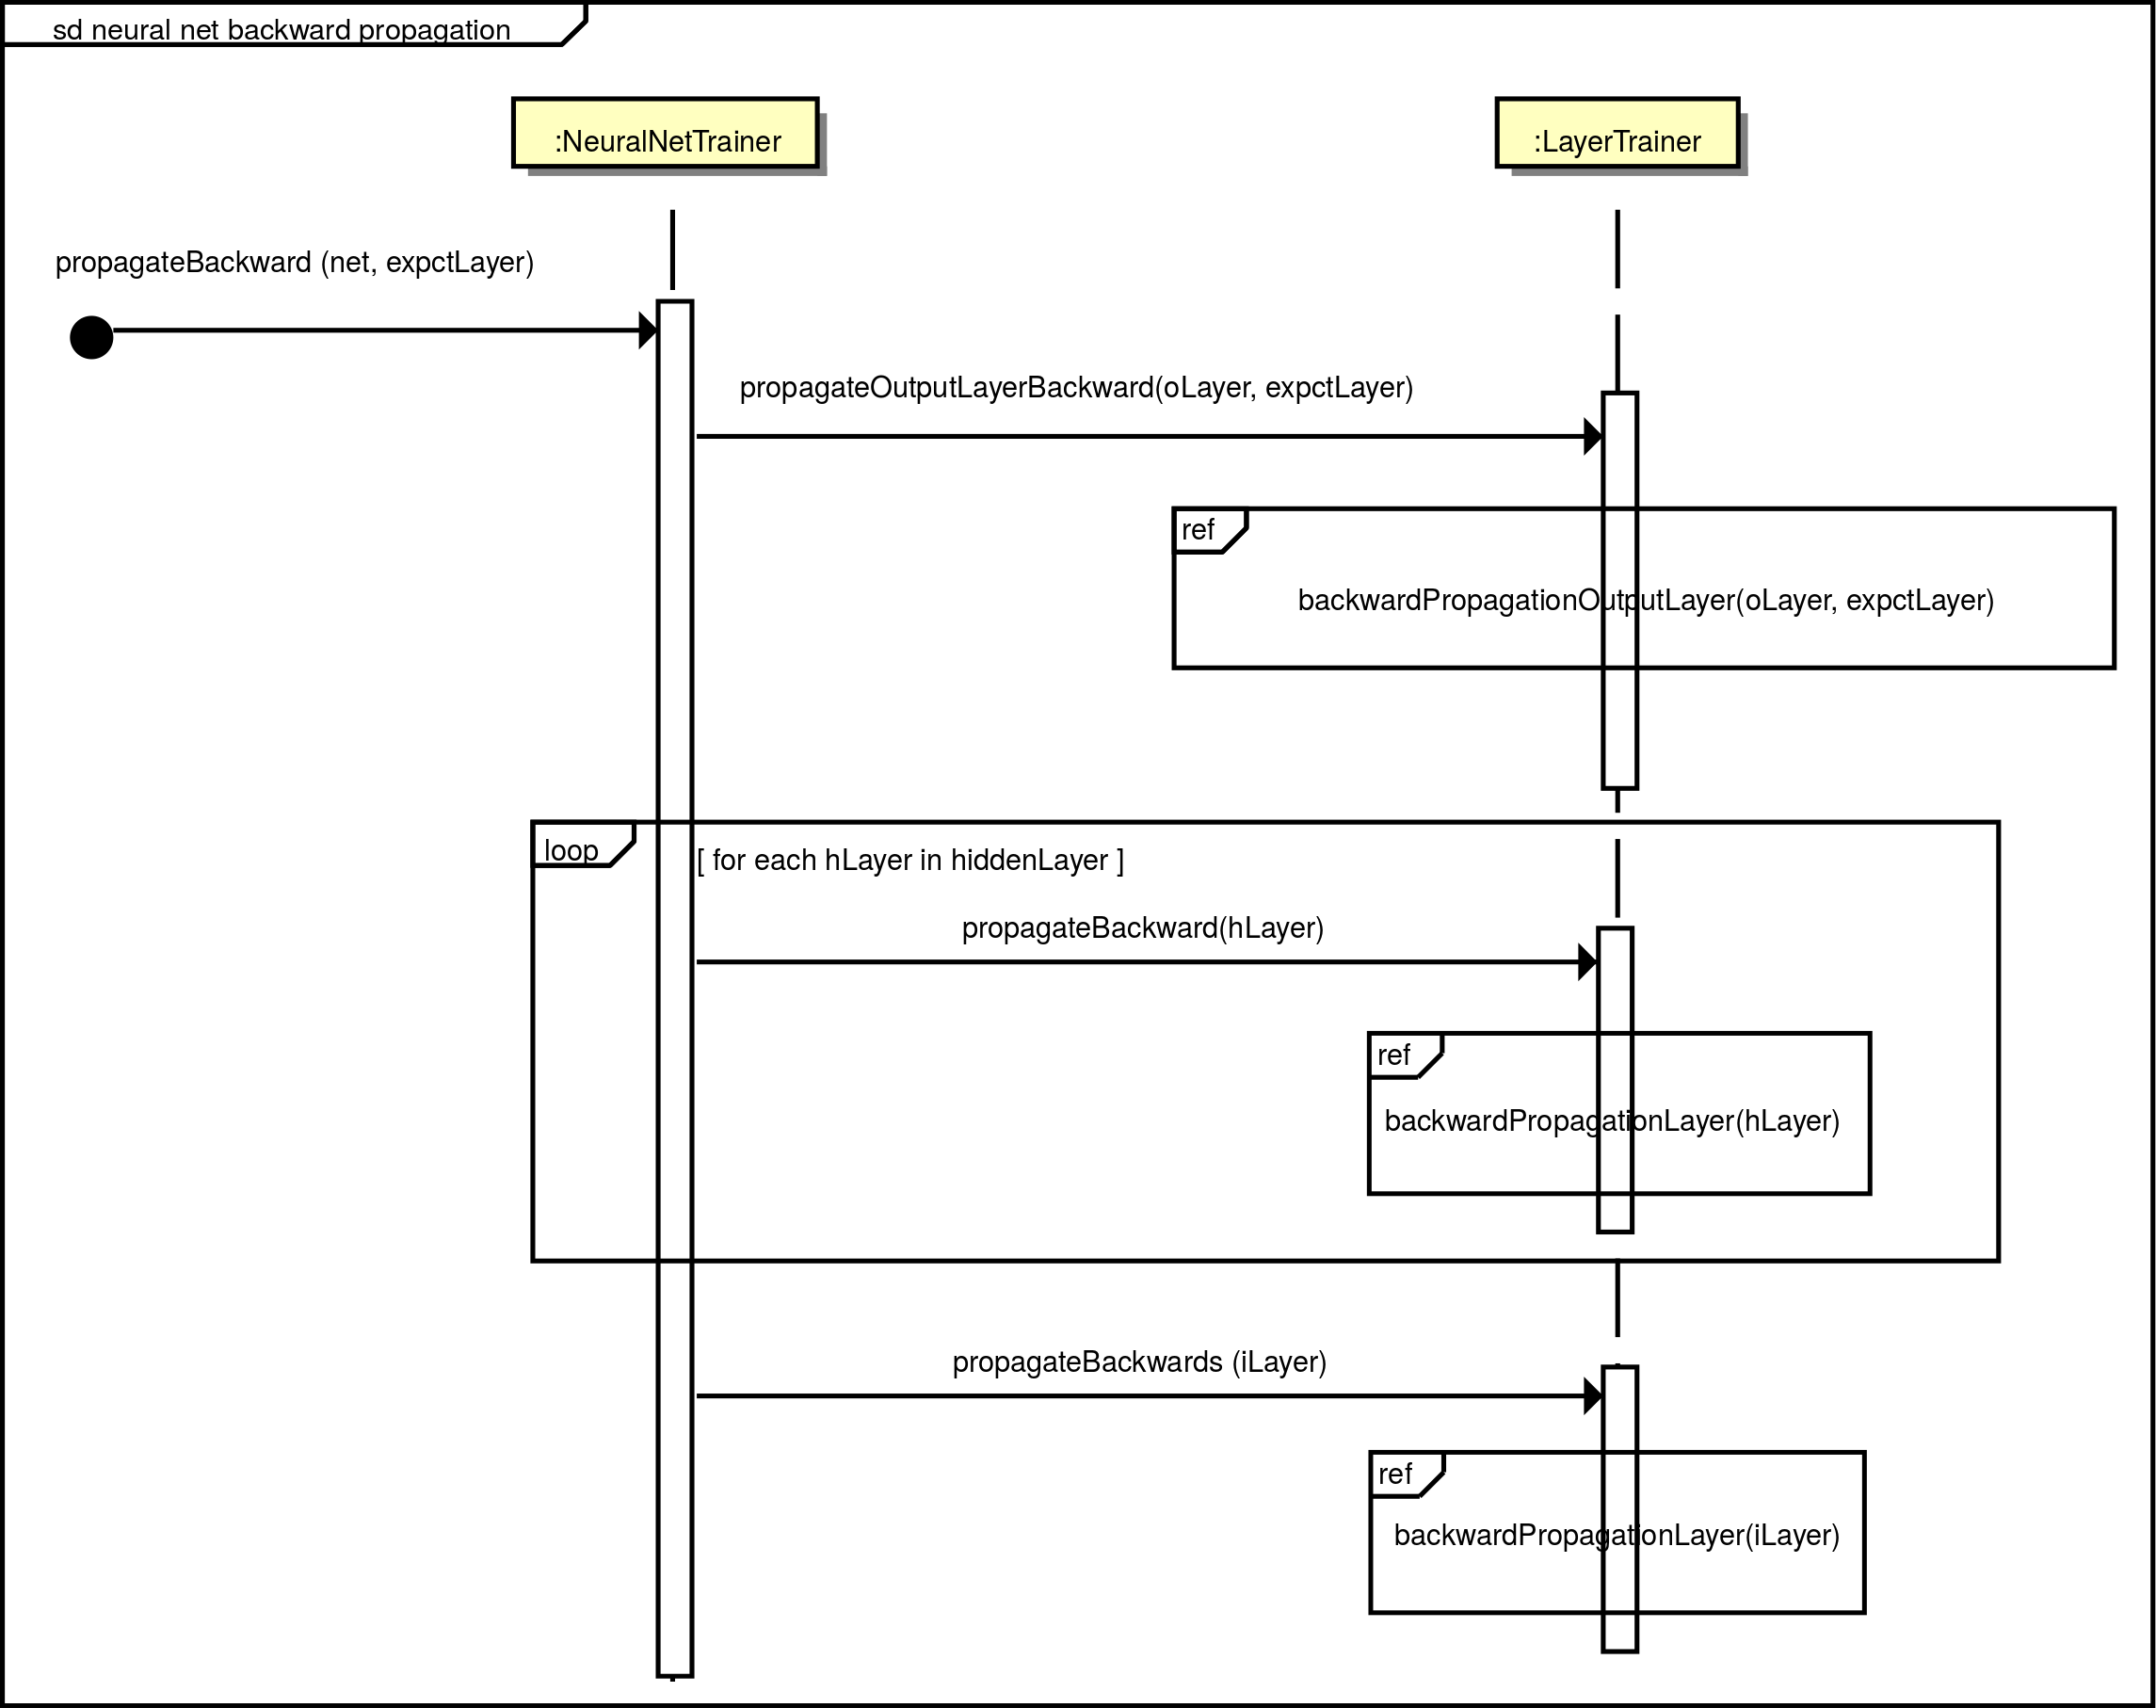
\includegraphics[width=15cm]{Abbildungen/UML/jan/gradientdescent1.png}
\caption{Sequenzdiagramm zur Backpropagation beginnend beim neuronalen Netz.}
\label{fig_sdBackpropagation}
\end{center}
\end{figure}

\textbf{/F301/} 
\begin{figure}[H]
\begin{center}
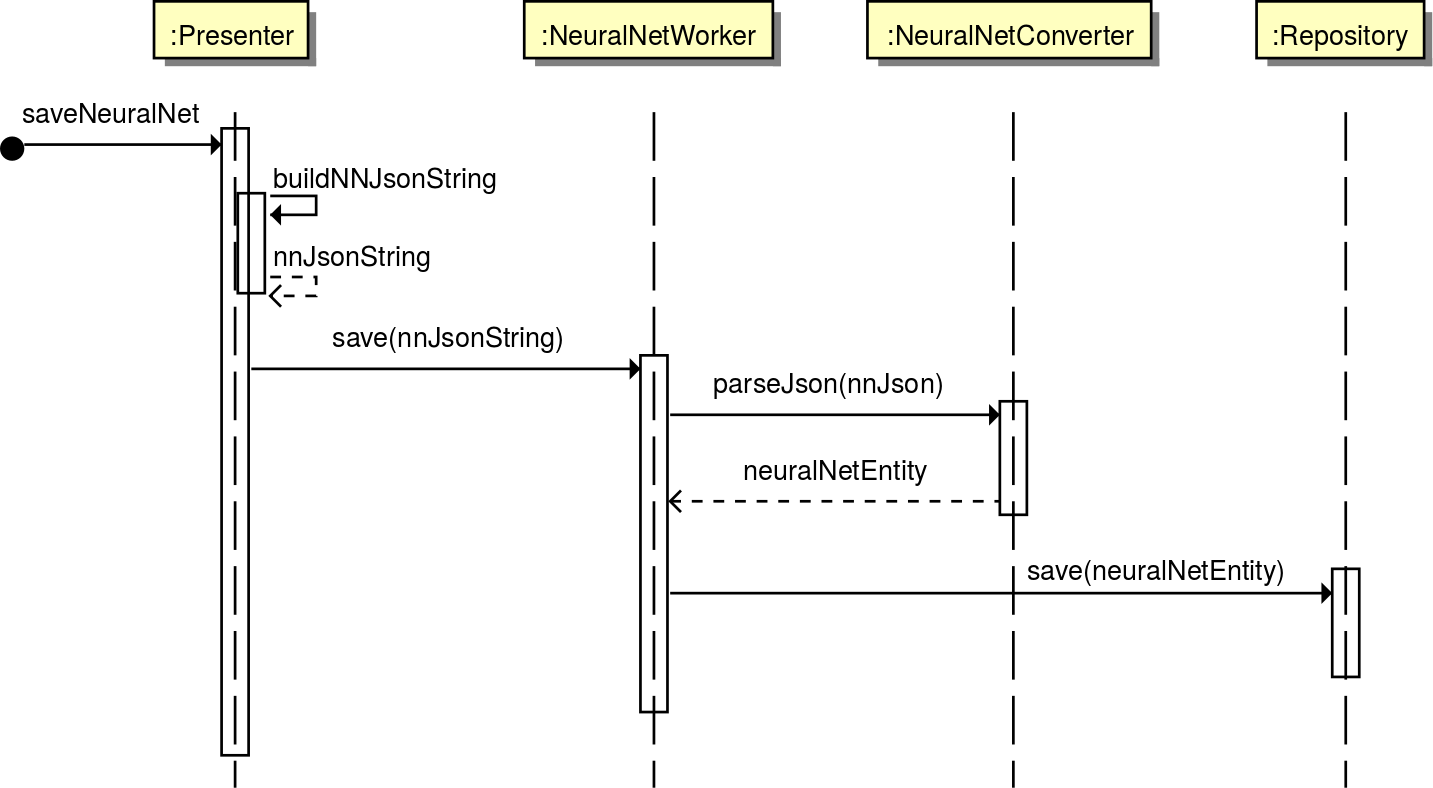
\includegraphics[width=15cm]{Abbildungen/UML/jan/convertJsonNNSD.png}
\caption{Sequenzdiagramm zur Konvertierung eines JSON-Strings in ein neuronalen Netz.}
\label{fig_sdBackpropagation}
\end{center}
\end{figure}

\chapter{Daten}

\section{Datenstrukturen zur Persistenz eines Neuronalen Netzes}

Jedes Neuronale Netz wird zur Persistenz auf die unten dargestellten Datenstrukturen abgebildet, welche dann in der MongoDB abgelegt werden. 
\begin{figure}[h]
\begin{center}
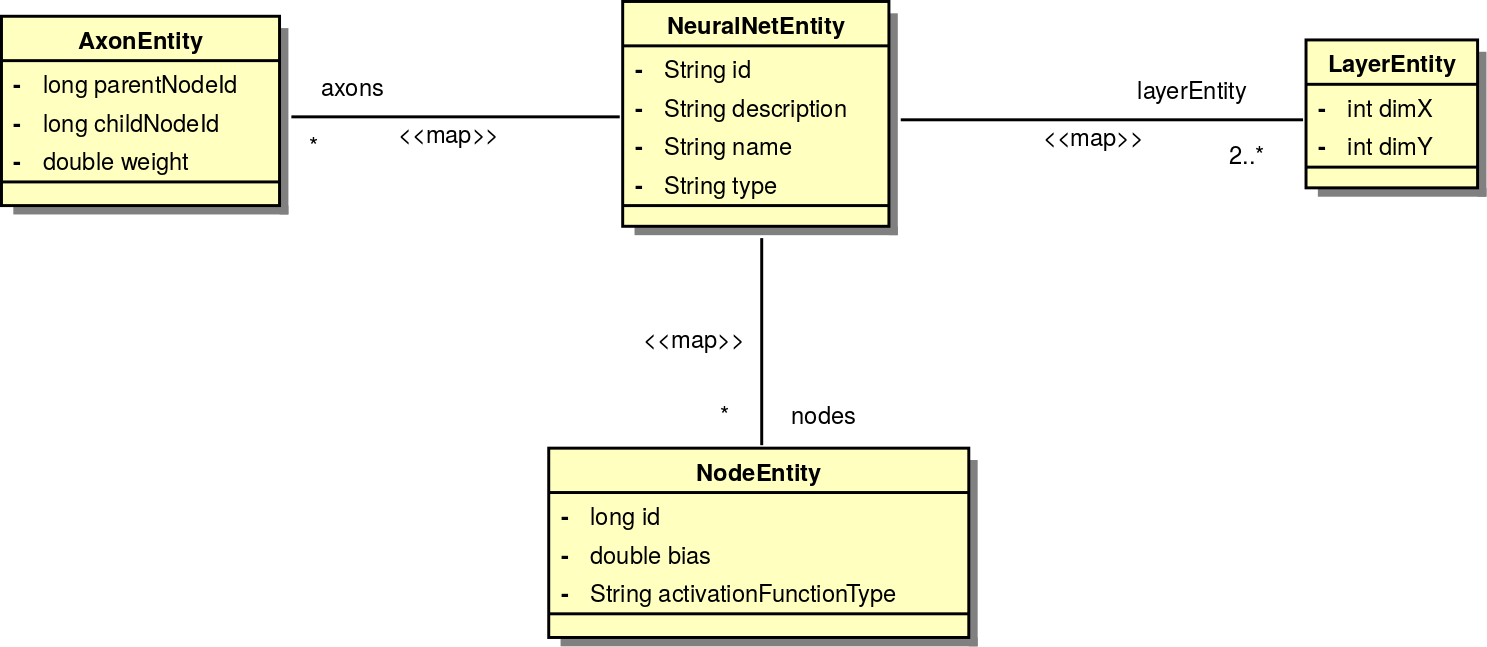
\includegraphics[width=\textwidth]{Abbildungen/UML/jan/datenBankKlassendiagramm.png}
\end{center}
\end{figure}
Es ist zu beachten, dass die Objekt dabei nicht als unabhängige, in Beziehung stehende Entitäten\footnote{Dies entspräche dem Vorgehen für eine Relationale Datenbank. Durch die vielen zirkulären Referenzen ist dieser Zugang nicht geeignet} in der Datenbank sondern als ein einziges Json-Objekt abgelegt werden. 
 
\chapter{Leistungen}
Leistungen: Anforderungen bezüglich Zeit und Genauigkeit
 
 
\chapter{Leistungen}
Leistungen: Anforderungen bezüglich Zeit und Genauigkeit
 
\chapter{Benutzungsoberfläche}
Benutzungsoberfläche: grundlegende Anforderungen, Zugriffsrechte
 
\begin{figure}[ht]
  \centering
  \rule{8cm}{6cm}
  \caption{Dies könnte ein Bild der Benutzungsoberfläche sein}
\end{figure}
 
\chapter{Qualitätsziele}
Qualiätsziele: Allgemeine Ziele sind meistens Änderbarkeit und Wartbarkeit.
Ziele sollten jedoch grundsätzlich messbar, spezifisch und relevant sein.
 
\chapter{Ergänzungen}
Hier ist Platz für nicht im Pflichtenheft abgedeckte Themengebiete oder ein
Glossar.
 
% Abbildungsverzeichnis
\listoffigures
 
\end{document}
